\documentclass[12pt,a4paper]{article}
\usepackage[margin=2.5cm]{geometry}
\usepackage{booktabs,longtable,array,tabularx}
\usepackage{amsmath,amssymb}
\usepackage{graphicx}
\usepackage{hyperref}
\usepackage{float}
\usepackage{microtype}
\usepackage{parskip}
\usepackage{caption}
\usepackage{xcolor}
\usepackage{enumitem}
\hypersetup{colorlinks=true,linkcolor=blue,urlcolor=blue}
\captionsetup{font=small,labelfont=bf}

\title{\textbf{BRSM Movie Memory Experiment}\\
\large Comprehensive Statistical Report\\
\normalsize After Vigilance-Based and Repeated-Video Exclusions}
\author{RSS Team}
\date{April 2026}

\begin{document}
\maketitle
\tableofcontents
\newpage


\section{Overview and Data Quality}

\subsection{Experiment Description}
The BRSM Movie Memory Experiment investigates how the type of event boundaries (Natural vs. Abrupt) encountered during video encoding influences subsequent recognition memory. Participants viewed a series of video clips and later completed a recognition task. The goal is to determine if abrupt edits disrupt boundary-related memory retrieval more than natural transitions.

\subsection{Vigilance-based exclusions}
Two participants failed the embedded vigilance check and are excluded from every analysis:
\begin{itemize}[nosep]
  \item \texttt{sub105\_AB}
  \item \texttt{sub70\_NB}
\end{itemize}

\subsection{Repeated-video exclusion}
Five movies per condition (IDs 3, 7, 18, 28, 37) were presented \emph{twice} during
encoding as attention checks. All recognition trials corresponding to these repeated movies
are excluded from every analysis. \textbf{Rationale:} participants received two encoding
exposures for these clips; their recognition performance is therefore not comparable to
single-exposure movies and would artificially inflate accuracy estimates.


\subsection{Sample and trial structure}
The retained analytical sample is $N=168$ (NB=88, AB=80),
contributing 5,880 recognition trials (35 unique movies $\times$ 168 participants).

\begin{table}[H]
\centering
\begin{tabular}{lrrrrr}
\hline
\textbf{Condition} & \textbf{n} & \textbf{n trials} & \textbf{BB trials} & \textbf{EM trials} \\
\hline
NB (Natural Boundary) & 88 & 3,080 & 1540 & 1540 \\
AB (Abrupt Boundary)  & 80 & 2,800 & 1400 & 1400 \\
Total & 168 & 5,880 & --- & --- \\
\hline
\end{tabular}
\caption{Analytical sample after all exclusions (35 unique movies per participant).}
\end{table}


\section{Statistical Methods}

Each hypothesis follows an identical pre-specified decision pipeline:
\begin{enumerate}[nosep]
  \item Build the DV at the participant level from trial-level data.
  \item Compute full descriptive statistics ($n$, $M$, $SD$, $Mdn$, $Q_1$, $Q_3$, min, max) per group.
  \item Test normality within each group using the Shapiro--Wilk test ($\alpha = .05$).
  \item Test variance homogeneity using Levene's test (median-centred; Brown--Forsythe variant).
  \item Select the inferential test:
    \begin{itemize}[nosep]
      \item Both groups normal \emph{and} equal variance $\Rightarrow$ Student's $t$-test
      \item Both groups normal \emph{and} unequal variance $\Rightarrow$ Welch's $t$-test
      \item Either group non-normal $\Rightarrow$ Mann--Whitney $U$ test (two-sided)
    \end{itemize}
  \item Report effect sizes: Cohen's $d$ / Hedges' $g$ for parametric tests;
        rank-biserial $r$ for non-parametric tests.
\end{enumerate}
No correction for multiple comparisons is applied. All reported $p$-values are raw.

\subsection{Accuracy dependent variable}
All accuracy-based DVs use raw proportion correct (range 0--1). Chance performance is 0.5
in a two-alternative forced-choice task. After excluding 5 repeated movies per participant,
each participant contributes 35 unique-movie trials (approximately 17--18 BB + 17--18 EM).

\subsection{Log-transformation and normality of response time}

Trial-level RTs are strongly right-skewed (skew $\approx 3.85$, excess kurtosis $\approx 32.50$). All RT analyses therefore use natural-log-transformed RT (ln seconds).
Table~\ref{tab:rt_normality} verifies that the transform rescues approximate normality
at the participant level.

\begin{table}[H]
\centering
\small
\begin{tabular}{llrrl}
\hline
\textbf{Condition} & \textbf{Transform} & \textbf{n} & \textbf{M} & \textbf{Shapiro--Wilk $p$} \\
\hline
NB & Raw RT (s) & 88 & 5.883 s & $<.001$ (non-normal) \\
   & Log RT (ln s) & 88 & 1.626 & $.5024$ (normal) \\
AB & Raw RT (s) & 80 & 5.708 s & $<.001$ (non-normal) \\
   & Log RT (ln s) & 80 & 1.595 & $.0746$ (normal) \\
All (trial) & Raw RT & 5000 sample & skew$=3.853$ & $<.001$ \\
            & Log RT & 5000 sample & skew$=0.588$ & $<.001$ \\
\hline
\end{tabular}
\caption{Shapiro--Wilk normality: raw RT vs.\ log RT at participant level (repeated movies excluded).}
\label{tab:rt_normality}
\end{table}

\noindent\textit{Note.} At the trial level ($n \approx 5,880$) Shapiro--Wilk has extreme power and flags even trivial departures from normality. The skew drops substantially after log-transformation, confirming normalisation. At the participant level both conditions pass after log-transformation.


\section{H1: Overall Recognition Accuracy}

\subsection{Hypotheses}

$H_0$: Overall recognition accuracy does not differ between Natural Boundary and Abrupt Boundary participants ($\mu_{\text{NB}} = \mu_{\text{AB}}$).

$H_1$: NB participants have higher overall recognition accuracy than AB participants ($\mu_{\text{NB}} > \mu_{\text{AB}}$; directional).

\subsection{DV and descriptive statistics}

\textbf{DV:} Per-participant proportion correct across all 35 unique recognition trials (repeated movies excluded).


\begin{table}[h!]
\centering
\small
\begin{tabular}{lrrrrrrrr}
\hline
\textbf{Group} & \textbf{n} & \textbf{M} & \textbf{SD} & \textbf{Mdn} & \textbf{Q1} & \textbf{Q3} & \textbf{Min} & \textbf{Max} \\
\hline
    NB & 88 & 0.867 & 0.075 & 0.886 & 0.829 & 0.921 & 0.629 & 1.000 \\
    AB & 80 & 0.832 & 0.084 & 0.829 & 0.771 & 0.886 & 0.571 & 1.000 \\
\hline
\end{tabular}
\caption{Descriptive statistics --- H1 (Overall accuracy).}
\label{tab:h1_desc}
\end{table}

\subsection{Test selection and result}

\textbf{Normality (Shapiro--Wilk):} NB $p = .0028$; AB $p = .0343$. At least one group rejects normality.

\textbf{Variance homogeneity (Levene):} $p = .3803$. Equal variances assumed.


\textbf{Test selected:} Mann--Whitney $U$. Tied ranks: 12 groups from 16 distinct values (tie correction $= 0.9865$, negligible).

\textbf{Result:} $U = 4384.500$, $p_{\text{one-sided}} = .0029$. Rank-biserial r $= 0.246$.

\textbf{Decision:} \textbf{Reject H\textsubscript{0}}. NB participants have significantly higher overall accuracy.


\section{H2: Before-Boundary Frame Accuracy}

\subsection{Hypotheses}

$H_0$: Recognition accuracy for Before-Boundary targets does not differ between conditions ($\mu_{\text{NB}} = \mu_{\text{AB}}$).

$H_1$: NB participants have higher Before-Boundary accuracy than AB participants ($\mu_{\text{NB}} > \mu_{\text{AB}}$; directional).

\subsection{DV and descriptive statistics}

\textbf{DV:} Per-participant proportion correct on BB-frame targets only (approximately 17--18 trials after exclusions).


\begin{table}[h!]
\centering
\small
\begin{tabular}{lrrrrrrrr}
\hline
\textbf{Group} & \textbf{n} & \textbf{M} & \textbf{SD} & \textbf{Mdn} & \textbf{Q1} & \textbf{Q3} & \textbf{Min} & \textbf{Max} \\
\hline
    NB & 88 & 0.854 & 0.100 & 0.889 & 0.778 & 0.944 & 0.556 & 1.000 \\
    AB & 80 & 0.808 & 0.115 & 0.833 & 0.722 & 0.889 & 0.389 & 1.000 \\
\hline
\end{tabular}
\caption{Descriptive statistics --- H2 (BB accuracy).}
\label{tab:h2_desc}
\end{table}

\subsection{Test selection and result}

\textbf{Normality (Shapiro--Wilk):} NB $p = <.001$; AB $p = <.001$. At least one group rejects normality.

\textbf{Variance homogeneity (Levene):} $p = .4261$. Equal variances assumed.


\textbf{Test selected:} Mann--Whitney $U$. Tied ranks: 9 groups from 11 distinct values (tie correction $= 0.9729$, negligible).

\textbf{Result:} $U = 4370.000$, $p_{\text{one-sided}} = .0031$. Rank-biserial r $= 0.241$.

\textbf{Decision:} \textbf{Reject H\textsubscript{0}}. NB participants recognise BB-frame targets significantly more accurately.


\section{H3: Mean Confidence Rating}

\subsection{Hypotheses}

$H_0$: Mean confidence rating does not differ between NB and AB participants ($\mu_{\text{NB}} = \mu_{\text{AB}}$).

$H_1$: NB participants report higher mean confidence than AB participants ($\mu_{\text{NB}} > \mu_{\text{AB}}$; directional).

\subsection{DV and descriptive statistics}

\textbf{DV:} Per-participant mean confidence rating (1--5 Likert scale; repeated movies excluded).


\begin{table}[h!]
\centering
\small
\begin{tabular}{lrrrrrrrr}
\hline
\textbf{Group} & \textbf{n} & \textbf{M} & \textbf{SD} & \textbf{Mdn} & \textbf{Q1} & \textbf{Q3} & \textbf{Min} & \textbf{Max} \\
\hline
    NB & 88 & 4.177 & 0.422 & 4.243 & 3.907 & 4.521 & 2.971 & 5.000 \\
    AB & 80 & 4.040 & 0.476 & 4.043 & 3.650 & 4.407 & 2.829 & 4.886 \\
\hline
\end{tabular}
\caption{Descriptive statistics --- H3 (Mean confidence).}
\label{tab:h3_desc}
\end{table}

\subsection{Test selection and result}

\textbf{Normality (Shapiro--Wilk):} NB $p = .0312$; AB $p = .1607$. At least one group rejects normality.

\textbf{Variance homogeneity (Levene):} $p = .1211$. Equal variances assumed.


\textbf{Test selected:} Mann--Whitney $U$. Tied ranks: 46 groups from 58 distinct values (tie correction $= 0.9994$, negligible).

\textbf{Result:} $U = 4097.500$, $p_{\text{one-sided}} = .0334$. Rank-biserial r $= 0.164$.

\textbf{Decision:} \textbf{Reject H\textsubscript{0}}. NB participants report significantly higher mean confidence.


\section{H4: Proportion of Low-Confidence Trials}

\subsection{Hypotheses}

$H_0$: The proportion of trials with confidence $\leq 3$ does not differ between conditions ($\pi_{\text{AB}} = \pi_{\text{NB}}$).

$H_1$: AB participants have a higher proportion of low-confidence trials ($\pi_{\text{AB}} > \pi_{\text{NB}}$; directional).

\subsection{DV and descriptive statistics}

\textbf{DV:} Per-participant proportion of trials rated confidence $\leq 3$ (repeated movies excluded).


\begin{table}[h!]
\centering
\small
\begin{tabular}{lrrrrrrrr}
\hline
\textbf{Group} & \textbf{n} & \textbf{M} & \textbf{SD} & \textbf{Mdn} & \textbf{Q1} & \textbf{Q3} & \textbf{Min} & \textbf{Max} \\
\hline
    AB & 80 & 0.277 & 0.153 & 0.286 & 0.164 & 0.400 & 0.000 & 0.657 \\
    NB & 88 & 0.243 & 0.132 & 0.229 & 0.143 & 0.343 & 0.000 & 0.629 \\
\hline
\end{tabular}
\caption{Descriptive statistics --- H4 (Low-confidence proportion).}
\label{tab:h4_desc}
\end{table}

\subsection{Test selection and result}

\textbf{Normality (Shapiro--Wilk):} AB $p = .1431$; NB $p = .0711$. Both groups pass normality.

\textbf{Variance homogeneity (Levene):} $p = .0922$. Equal variances assumed.


\textbf{Test selected:} Student's independent-samples t-test.

\textbf{Result:} $t = 1.577$, $df = 166$, $p_{\text{one-sided}} = .0584$. Cohen's d (pooled) $= 0.244$.

\textbf{Decision:} Fail to reject H\textsubscript{0}. AB participants show numerically more low-confidence responses.


\section{H5: Per-Movie Accuracy Variability}

\subsection{Hypotheses}

$H_0$: The standard deviation of per-movie accuracy does not differ between conditions ($\sigma_{\text{AB}} = \sigma_{\text{NB}}$).

$H_1$: AB participants show greater variability in per-movie accuracy ($\sigma_{\text{AB}} > \sigma_{\text{NB}}$; directional).

\subsection{DV and descriptive statistics}

\textbf{DV:} Per-participant standard deviation of accuracy across the 35 unique movies (repeated movies excluded).


\begin{table}[h!]
\centering
\small
\begin{tabular}{lrrrrrrrr}
\hline
\textbf{Group} & \textbf{n} & \textbf{M} & \textbf{SD} & \textbf{Mdn} & \textbf{Q1} & \textbf{Q3} & \textbf{Min} & \textbf{Max} \\
\hline
    AB & 80 & 0.360 & 0.085 & 0.382 & 0.323 & 0.426 & 0.000 & 0.502 \\
    NB & 88 & 0.324 & 0.089 & 0.323 & 0.272 & 0.382 & 0.000 & 0.490 \\
\hline
\end{tabular}
\caption{Descriptive statistics --- H5 (Per-movie accuracy SD).}
\label{tab:h5_desc}
\end{table}

\subsection{Test selection and result}

\textbf{Normality (Shapiro--Wilk):} AB $p = <.001$; NB $p = .0017$. At least one group rejects normality.

\textbf{Variance homogeneity (Levene):} $p = .5266$. Equal variances assumed.


\textbf{Test selected:} Mann--Whitney $U$. Tied ranks: 12 groups from 16 distinct values (tie correction $= 0.9865$, negligible).

\textbf{Result:} $U = 4428.000$, $p_{\text{one-sided}} = .0019$. Rank-biserial r $= 0.258$.

\textbf{Decision:} \textbf{Reject H\textsubscript{0}}. AB participants show significantly greater per-movie accuracy variability.


\section{H6: BB-Frame vs EM-Frame Response Time}

\subsection{Hypotheses}
$H_0$: Mean log RT does not differ between BB-frame and EM-frame recognition trials
($\mu_\text{BB} = \mu_\text{EM}$).

$H_1$: Mean log RT differs between BB-frame and EM-frame recognition trials
($\mu_\text{BB} \neq \mu_\text{EM}$; non-directional).

\textit{Rationale.} If BB-frame targets engage a qualitatively different retrieval process
(e.g., recollection rather than familiarity), recognition decisions for BB targets may take
longer than for EM targets. This within-participant comparison is exploratory and non-directional.

\subsection{DV and descriptive statistics}
DV: Per-participant mean log RT on BB trials and mean log RT on EM trials; the within-participant
difference BB$-$EM is tested against zero (repeated movies excluded).

\begin{table}[H]
\centering
\small
\begin{tabular}{lrrrrrrrr}
\hline
\textbf{Measure} & \textbf{n} & \textbf{M} & \textbf{SD} & \textbf{Mdn} & \textbf{Q1} & \textbf{Q3} & \textbf{Min} & \textbf{Max} \\
\hline
BB mean log RT (ln s) & 168 & 1.635 & 0.243 & 1.615 & 1.491 & 1.756 & 1.045 & 2.340 \\
EM mean log RT (ln s) & 168 & 1.586 & 0.246 & 1.596 & 1.416 & 1.741 & 1.029 & 2.290 \\
BB$-$EM difference    & 168 & 0.048 & 0.148 & 0.054 & -0.045 & 0.160 & -0.329 & 0.426 \\
\hline
\end{tabular}
\caption{Descriptive statistics --- H6 (BB vs EM log RT, within-participant).}
\end{table}

\subsection{Test selection and result}
\textbf{Normality of differences (Shapiro--Wilk):} $p = .6268$
(normal). One-sample $t$-test on differences is used.

\textbf{Test selected:} One-sample t-test on differences (paired, two-tailed).

\textbf{Result:} $t = 4.256$
, $df = 167$
, $p_{\text{two-sided}} = <.001$. Effect: Cohen's d\_z $= 0.328$.

\textbf{Decision:} Reject $H_0$.
BB-frame recognition decisions take significantly longer than EM-frame decisions
(mean difference $= 0.048$ ln s), consistent with a more effortful retrieval process for boundary-region events.


\section{H7: Mean log RT vs Overall Accuracy}

\subsection{Hypotheses}
$H_0$: There is no linear association between mean response time and overall recognition accuracy
($\rho = 0$; two-tailed).

$H_1$: There is a significant association between mean response time and overall recognition
accuracy ($\rho \neq 0$; two-tailed).

\textit{Rationale.} Slower responses on a recognition task could reflect greater uncertainty and
more effortful retrieval, which may be associated with lower accuracy (speed--accuracy trade-off).
Alternatively, slower, more careful responding could improve accuracy. The direction is not
pre-specified; the test is two-tailed.

\subsection{DV and descriptive statistics}
DV: Per-participant mean log RT (ln s) and per-participant overall accuracy (proportion correct
across all 35 unique trials; repeated movies excluded). Log RT is used because raw RT is
right-skewed (see \S2.3).

\begin{table}[H]
\centering
\small
\begin{tabular}{lrrrrrrrr}
\hline
\textbf{Variable} & \textbf{n} & \textbf{M} & \textbf{SD} & \textbf{Mdn} & \textbf{Q1} & \textbf{Q3} & \textbf{Min} & \textbf{Max} \\
\hline
Mean log RT (ln s) & 168 & 1.611 & --- & --- & --- & --- & --- & --- \\
Overall accuracy   & 168 & 0.851 & --- & --- & --- & --- & --- & --- \\
\hline
\end{tabular}
\caption{Descriptive statistics --- H7 (Mean log RT and Overall accuracy).}
\end{table}

\subsection{Test selection and result}
\textbf{Normality (Shapiro--Wilk):} Mean log RT: $W = 0.982$, $p = .0262$; Overall accuracy: $W = 0.960$, $p = <.001$.

\textbf{Test selected:} Spearman rank correlation (at least one variable non-normal; two-tailed). 95\% CI obtained by bootstrap ($B = 5000$).

\textbf{Result:} $\rho = -0.036$ ($n = 168$, $df = 166$), $p_{\text{two-sided}} = .6429$, 95\% CI $[-0.196,\, 0.116]$.

\textbf{Decision:} Fail to reject $H_0$.
No significant correlation was found between mean log RT and overall accuracy ($\rho = -0.036$, $p = .6429$).


\begin{figure}[H]
\centering
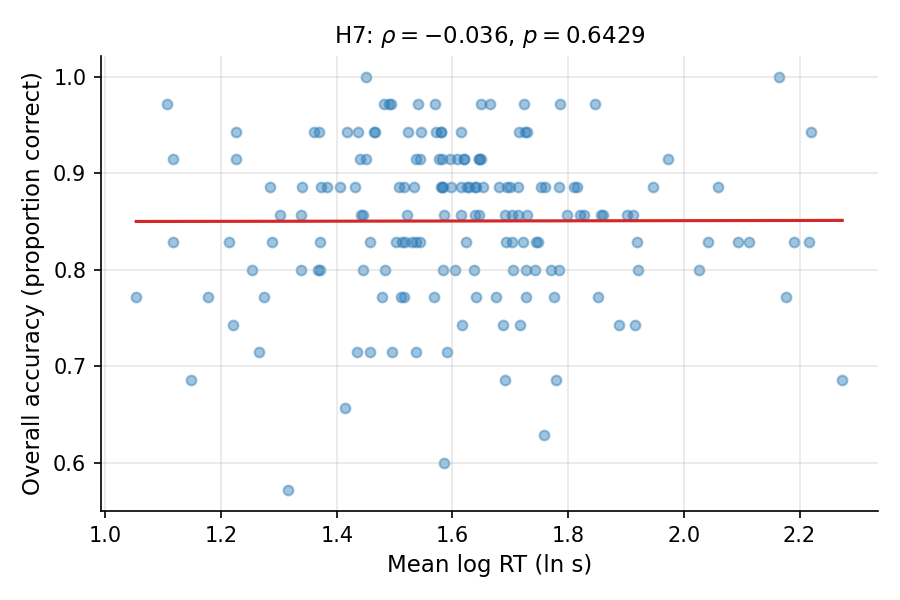
\includegraphics[width=0.65\textwidth]{h7_scatter.png}
\caption{H7 scatter plot: per-participant mean log RT vs.\ overall recognition accuracy (repeated movies excluded). Regression line added.}
\end{figure}


\section{H8: Mean log RT vs Mean Confidence Rating}

\subsection{Hypotheses}
$H_0$: There is no linear association between mean response time and mean confidence rating
($\rho = 0$; two-tailed).

$H_1$: There is a significant association between mean response time and mean confidence rating
($\rho \neq 0$; two-tailed).

\textit{Rationale.} High confidence is associated with fast, fluent recognition (the `feeling
of knowing' literature), so slower mean RT may predict lower confidence. The direction is not
pre-specified; the test is two-tailed.

\subsection{DV and descriptive statistics}
DV: Per-participant mean log RT (ln s) and per-participant mean confidence rating (1--5 Likert
scale). Log RT is used for the same reason as H7. Repeated movies are excluded.

\subsection{Test selection and result}
\textbf{Normality (Shapiro--Wilk):} Mean log RT: $p = .0262$; Mean confidence: $p = .0053$.

\textbf{Test selected:} Spearman rank correlation (at least one variable non-normal; two-tailed). 95\% CI obtained by bootstrap ($B = 5000$).

\textbf{Result:} $\rho = -0.163$ ($n = 168$, $df = 166$), $p_{\text{two-sided}} = .0342$, 95\% CI $[-0.313,\, -0.005]$.

\textbf{Decision:} Reject $H_0$.
A statistically significant negative Spearman correlation was found between mean log RT and mean confidence rating ($\rho = -0.163$, $p = .0342$).


\begin{figure}[H]
\centering
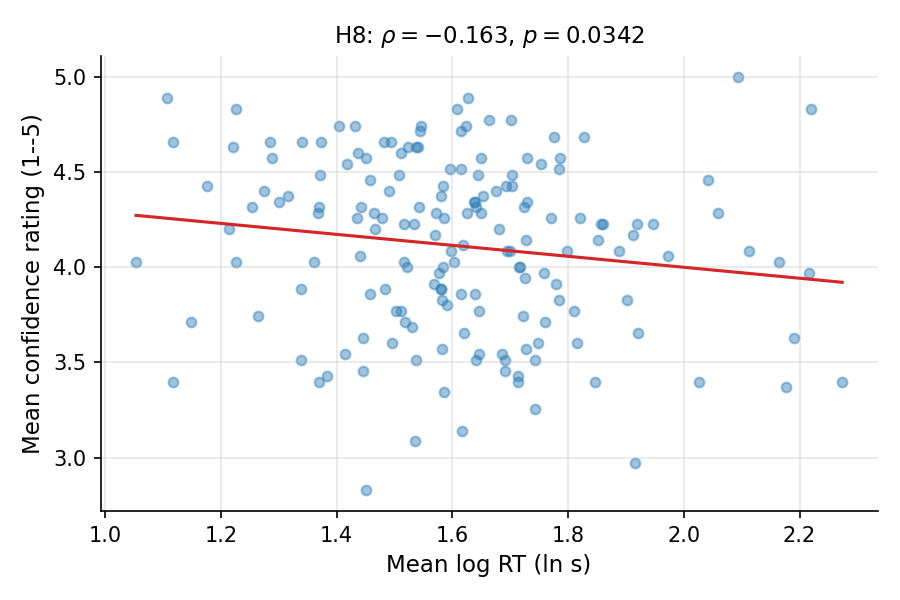
\includegraphics[width=0.65\textwidth]{h8_scatter.png}
\caption{H8 scatter plot: per-participant mean log RT vs.\ mean confidence rating (repeated movies excluded). Regression line added.}
\end{figure}


\section{Regression Analysis}

\subsection{Overview and Feature Policy}
A strict regression pipeline was applied to predict trial-level recognition accuracy
(\texttt{resp.corr}, binary) from pre-response design variables and pre-treatment participant
covariates. Post-response variables (RT, confidence) were explicitly excluded to prevent data
leakage. Two participants who failed the vigilance check are excluded throughout. All trials
from the five repeated movies are excluded (is\_repeat = 0 only); because no repeated trials
remain, \texttt{is\_repeat} is not a predictor in any model.

\begin{itemize}[nosep]
  \item \textbf{Included (pre-response):} condition, target\_type, movie\_duration, stimulus\_id
  \item \textbf{Optional controls (pre-treatment):} age, gender, handedness, vision
  \item \textbf{Excluded (leakage / post-response):} resp.rt, conf\_radio.response
  \item \textbf{Excluded (zero-variance after filtering):} is\_repeat
\end{itemize}

Three complementary models are used:
\begin{enumerate}[nosep]
  \item \textbf{Model~3} --- participant-level binomial GLM
  \item \textbf{Model~1} --- trial-level GEE logistic regression (8 nested models)
  \item \textbf{GLMM}    --- trial-level binomial mixed model with random participant intercept (Variational Bayes)
\end{enumerate}

\subsection{Model 3: Participant-Level Binomial GLM}
A participant-level binomial GLM (link: logit) was fitted with condition, age, and gender as
predictors, using (successes, failures) counts as the response.

\begin{table}[H]
\centering
\small
\begin{tabular}{lrrrl}
\hline
\textbf{Term} & \textbf{Coef} & \textbf{$p$} & \textbf{OR} \\
\hline

    const & 2.711 & $<.001$ & 15.047 \\

    age & -0.034 & $.0822$ & 0.967 \\

    condition\_AB & -0.339 & $<.001$ & 0.713 \\

    target\_type\_EM & 0.246 & $.0215$ & 1.279 \\

    gender\_Male & -0.248 & $.0064$ & 0.780 \\

    condition\_AB:target\_type\_EM & 0.109 & $.4631$ & 1.115 \\

\hline
\end{tabular}
\caption{Model 3 --- Participant-level binomial GLM: coefficients and odds ratios (repeated movies excluded).}
\end{table}


\noindent\textbf{Key finding:} NB condition significantly increases accuracy odds.
Male gender is associated with lower accuracy odds. Age shows a borderline negative effect.

\subsection{Model 1: Trial-Level GEE Logistic Regression}
Eight candidate GEE models (Binomial family, exchangeable working correlation, robust SE)
were fitted with trials clustered by participant. Models were compared by QIC (lower is better);
unstable models (non-finite parameters / SEs) were flagged and excluded from best-model selection.

\begin{table}[H]
\centering
\small
\begin{tabular}{llp{7cm}}
\hline
\textbf{Model} & \textbf{QIC} & \textbf{Description} \\
\hline

    M1\_stim\_interaction & 4889.55 & Interaction + demographics + stimulus duration. \\

    M1\_stim\_main & 4889.90 & Main effects + demographics + stimulus duration. \\

    M1\_demo\_interaction & 4909.07 & Interaction + demographics. \\

    M1\_demo\_main & 4909.37 & Main effects + demographics (age, gender, handedness, vision). \\

    M1\_core\_interaction & 4930.40 & Condition × target\_type interaction. The interaction term tests whether the BB-vs-EM accuracy difference is moderated by condition (NB vs AB). \\

    M1\_core\_main & 4930.71 & Main effects: condition + target\_type. \\

    M1\_movieFE\_interaction \textit{(unstable)} & --- & Interaction + movie fixed effects. \\

    M1\_movieFE\_main \textit{(unstable)} & --- & Main effects + demographics + duration + movie fixed effects. \\

\hline
\end{tabular}
\caption{Model 1 --- GEE model comparison by QIC (lower is better; repeated movies excluded).}
\end{table}

\subsection{Best Model: M1\_stim\_interaction --- Odds Ratios}

The best stable model by QIC is M1\_stim\_interaction.

\begin{table}[H]
\centering
\footnotesize
\begin{tabular}{lrrrrrr}
\hline
\textbf{Term} & \textbf{Coef} & \textbf{SE} & \textbf{$z$} & \textbf{$p$} & \textbf{OR} & \textbf{95\% CI} \\
\hline

    Intercept & 1.916 & 0.588 & 3.260 & $.0011$ & 6.796 & [2.148, 21.505] \\

    Condition: AB vs NB & -0.333 & 0.119 & -2.791 & $.0053$ & 0.717 & [0.567, 0.906] \\

    Target type: EM vs BB & 0.256 & 0.101 & 2.535 & $.0113$ & 1.292 & [1.060, 1.576] \\

    Gender: Male vs Female & -0.236 & 0.118 & -2.004 & $.0451$ & 0.790 & [0.627, 0.995] \\

    Handedness: Right & 0.269 & 0.249 & 1.078 & $.2811$ & 1.309 & [0.802, 2.134] \\

    Vision: Normal & 0.043 & 0.096 & 0.448 & $.6542$ & 1.044 & [0.864, 1.261] \\

    Vision: Uncorrected difficulty & 1.171 & 0.396 & 2.958 & $.0031$ & 3.224 & [1.484, 7.002] \\

    Condition(AB) $\times$ Target(EM) & 0.115 & 0.141 & 0.817 & $.4139$ & 1.122 & [0.851, 1.479] \\

    Age & -0.038 & 0.023 & -1.631 & $.1028$ & 0.963 & [0.920, 1.008] \\

    Movie duration (s) & 0.018 & 0.003 & 5.129 & $<.001$ & 1.018 & [1.011, 1.025] \\

\hline
\end{tabular}
\caption{Best GEE model: odds ratios with 95\% CI (repeated movies excluded).}
\end{table}


\subsection{Interaction Effects in the GEE Models}
\label{sec:interaction}

Several candidate models include a \textbf{condition $\times$ target\_type interaction}.
This section explains how to interpret these interaction terms.

\subsubsection{What the interaction term tests}

The term \texttt{C(condition)[T.AB]:C(target\_type)[T.EM]} tests whether the difference in
log-odds of a correct response between EM-frame and BB-frame targets is \emph{the same} in
both the AB and NB conditions.

Let $\beta_1$ = coefficient for condition (AB vs NB, reference = NB), $\beta_2$ = coefficient
for target type (EM vs BB, reference = BB), and $\beta_3$ = interaction coefficient. Then:
\begin{align*}
\text{NB} + \text{BB:} &\quad \alpha \quad \text{(reference cell)} \\
\text{NB} + \text{EM:} &\quad \alpha + \beta_2 \quad \text{(EM advantage in NB)} \\
\text{AB} + \text{BB:} &\quad \alpha + \beta_1 \quad \text{(AB penalty for BB targets)} \\
\text{AB} + \text{EM:} &\quad \alpha + \beta_1 + \beta_2 + \beta_3 \quad \text{(combined effects in AB)}
\end{align*}

So $\beta_3$ measures \textbf{how the EM advantage over BB changes} when moving from NB to AB.

\subsubsection{Interpreting the sign of the interaction}
\begin{itemize}[nosep]
  \item $\beta_3 > 0$ (OR $> 1$): the EM advantage is \emph{larger} in AB than in NB --- the AB condition hurts BB recall proportionally more than EM recall.
  \item $\beta_3 < 0$ (OR $< 1$): the EM advantage is \emph{smaller} in AB --- boundary disruption reduces BB and EM recognition approximately equally.
  \item $\beta_3 \approx 0$ (OR $\approx 1$): no moderation --- condition and frame type act independently.
\end{itemize}

\subsubsection{Odds ratios for interaction terms are ``ratios of odds ratios''}
The OR for the interaction is
$$\text{OR}_\text{interaction} = e^{\beta_3} = \frac{\text{OR}_{\text{EM/BB in AB}}}{\text{OR}_{\text{EM/BB in NB}}}.$$
This is not a standalone probability but the \emph{multiplicative change} in the EM advantage
when switching from NB to AB.

\subsubsection{Recovering simple (conditional) effects}
\begin{itemize}[nosep]
  \item Effect of \textbf{condition for BB targets:} $e^{\beta_1}$ \hfill (AB vs NB, BB trials only)
  \item Effect of \textbf{condition for EM targets:} $e^{\beta_1 + \beta_3}$ \hfill (AB vs NB, EM trials only)
  \item Effect of \textbf{target type in NB:} $e^{\beta_2}$ \hfill (EM vs BB, NB participants)
  \item Effect of \textbf{target type in AB:} $e^{\beta_2 + \beta_3}$ \hfill (EM vs BB, AB participants)
\end{itemize}
These simple effects answer: ``What is the effect of X when Y is held at a specific level?''

\subsubsection{GEE vs GLMM for interaction estimates}
GEE estimates \emph{population-average} ORs (``On average across all participants, how does condition moderate the frame-type effect?''), while GLMM estimates \emph{subject-specific} ORs (``For a given participant, how does condition moderate the effect?''). Both families should agree in sign and significance. A large discrepancy signals substantial between-participant heterogeneity in the moderation.

\subsection{Diagnostics}

\subsubsection{Collinearity (VIF)}

\begin{table}[H]
\centering
\small
\begin{tabular}{lr}
\hline
\textbf{Variable} & \textbf{VIF} \\
\hline

    const & 164.366 \\

    gender\_Male & 1.092 \\

    age & 1.090 \\

    vision\_Normal & 1.063 \\

    condition\_AB & 1.050 \\

    vision\_Uncorrected vision difficulty & 1.025 \\

    handedness\_Right handed & 1.017 \\

    movie\_duration & 1.002 \\

    target\_type\_EM & 1.002 \\

\hline
\end{tabular}
\caption{Variance inflation factors for trial-level predictors (VIF $< 5$ = acceptable).}
\end{table}


\subsubsection{Heteroscedasticity (Breusch--Pagan, OLS surrogate)}
A Breusch--Pagan test was run on an OLS surrogate model predicting participant-level accuracy
from condition, age, and gender. The primary Model~1 is logistic (GEE) and does not assume
homoscedasticity; this diagnostic is provided for completeness.

\begin{table}[H]
\centering
\small
\begin{tabular}{lrrrrrr}
\hline
\textbf{Model} & \textbf{BP LM} & \textbf{$p_\text{LM}$} & \textbf{BP F} & \textbf{$p_F$} & \textbf{n} & \textbf{$R^2$} \\
\hline
OLS accuracy & 2.633 & $.4517$ & 0.870 & $.4577$ & 168 & 0.083 \\
\hline
\end{tabular}
\caption{Breusch--Pagan heteroscedasticity test (OLS surrogate on participant accuracy).}
\end{table}

\noindent Both Breusch--Pagan statistics are non-significant ($p > .40$), indicating no evidence
of heteroscedasticity in the OLS surrogate.


\subsection{Mixed-Effects Logistic Regression (GLMM)}

\subsubsection{Rationale and Model Specification}
Because each participant completed 35 trials (after repeated-movie exclusion), observations are
not independent. A binomial mixed-effects logistic model addresses this by including a
\textbf{random intercept for participant\_id}, which controls for stable individual differences
in baseline recognition accuracy.

Estimation uses \textbf{Variational Bayes} (\texttt{statsmodels BinomialBayesMixedGLM.fit\_vb()}).
Variational Bayes is preferred over the Laplace approximation (\texttt{fit\_map}) because it
reliably estimates the random-effect variance in balanced designs; the Laplace approximation
can collapse the random-effect SD to zero in such cases.
Approximate $z$-statistics and $p$-values are derived from $z = \hat\beta / \text{Post.SD}$
using the standard normal distribution.

Three GLMM variants are reported:
\begin{enumerate}[nosep]
  \item \textbf{Core} (condition + target\_type main effects)
  \item \textbf{Interaction} (condition $\times$ target\_type)
  \item \textbf{Full} (condition + target\_type + age + gender + movie\_duration)
\end{enumerate}

\subsubsection{Fixed Effects}

\begin{table}[H]
\centering
\footnotesize
\begin{tabular}{lrrrrl}
\hline
\textbf{Predictor} & \textbf{Post.\ Mean} & \textbf{Post.\ SD} & \textbf{$z$} & \textbf{$p$ (approx)} & \textbf{OR} \\
\hline
    Intercept & 1.8201 & 0.0370 & 49.201 & $<.001$ & 6.1727 \\
    Condition: AB vs NB & -0.2851 & 0.0737 & -3.866 & $<.001$ & 0.7520 \\
    Target type: EM vs BB & 0.3110 & 0.0742 & 4.190 & $<.001$ & 1.3648 \\
\hline
\end{tabular}
\caption{GLMM core --- main effects (repeated movies excluded).}
\label{tab:glmm_core}
\end{table}

\begin{table}[H]
\centering
\footnotesize
\begin{tabular}{lrrrrl}
\hline
\textbf{Predictor} & \textbf{Post.\ Mean} & \textbf{Post.\ SD} & \textbf{$z$} & \textbf{$p$ (approx)} & \textbf{OR} \\
\hline
    Intercept & 1.8205 & 0.0370 & 49.201 & $<.001$ & 6.1750 \\
    Condition: AB vs NB & -0.3336 & 0.0738 & -4.523 & $<.001$ & 0.7163 \\
    Target type: EM vs BB & 0.2525 & 0.0743 & 3.401 & $<.001$ & 1.2872 \\
    Condition(AB) $\times$ Target(EM) & 0.1135 & 0.0888 & 1.279 & $.2010$ & 1.1202 \\
\hline
\end{tabular}
\caption{GLMM interaction --- condition $\times$ target\_type (repeated movies excluded).}
\label{tab:glmm_int}
\end{table}

\begin{table}[H]
\centering
\footnotesize
\begin{tabular}{lrrrrl}
\hline
\textbf{Predictor} & \textbf{Post.\ Mean} & \textbf{Post.\ SD} & \textbf{$z$} & \textbf{$p$ (approx)} & \textbf{OR} \\
\hline
    Intercept & 1.8333 & 0.0371 & 49.443 & $<.001$ & 6.2543 \\
    Condition: AB vs NB & -0.2969 & 0.0739 & -4.016 & $<.001$ & 0.7432 \\
    Target type: EM vs BB & 0.3247 & 0.0744 & 4.364 & $<.001$ & 1.3836 \\
    Gender: Male vs Female & -0.2539 & 0.0882 & -2.878 & $.0040$ & 0.7758 \\
    Age & -0.0378 & 0.0191 & -1.978 & $.0479$ & 0.9629 \\
    Movie duration (s) & 0.0182 & 0.0041 & 4.501 & $<.001$ & 1.0184 \\
\hline
\end{tabular}
\caption{GLMM full --- main effects + age + gender + movie\_duration (repeated movies excluded).}
\label{tab:glmm_full}
\end{table}


\subsubsection{Random Effects}
The random-effect standard deviation (SD) quantifies between-participant variability in
baseline log-odds accuracy, after accounting for fixed effects.

\begin{table}[H]
\centering
\small
\begin{tabular}{lrp{5.5cm}}
\hline
\textbf{GLMM variant} & \textbf{Random intercept SD} & \textbf{Interpretation} \\
\hline
Core (main effects) & 0.4203 & Between-participant variability in log-odds \\
Interaction & 0.4205 & Same, after adding interaction \\
Full (+ age, gender, duration) & 0.4016 & Same, after demographic controls \\
\hline
\end{tabular}
\caption{GLMM random intercept SDs (log-odds scale; repeated movies excluded).}
\end{table}

\noindent A random intercept SD of $\approx 0.42$ indicates meaningful between-person
variability in baseline recognition accuracy --- justifying the inclusion of random intercepts
per participant. The SD is stable across model variants, suggesting it is not confounded
with the fixed-effect predictors.


\subsubsection{Interaction Interpretation in the GLMM}

The interaction term in the GLMM (\texttt{C(condition)[T.AB]:C(target\_type)[T.EM]})
has the same structural interpretation as in the GEE (see \S\ref{sec:interaction}), but now
represents a \emph{subject-specific} (conditional) effect rather than a population-average effect.

The posterior mean of the interaction coefficient indicates whether the EM advantage over BB
is larger or smaller in the AB condition relative to NB, \emph{for a given participant} (after
integrating out individual differences via the random intercept).

Key comparison with GEE:
\begin{itemize}[nosep]
  \item If GEE and GLMM interaction ORs agree in sign and magnitude: the moderation is consistent across participants.
  \item If they diverge substantially: there is heterogeneity in how the condition moderates the frame-type effect across individuals.
\end{itemize}

\subsubsection{Summary}
The GLMM provides the most methodologically rigorous answer to the primary research question.
After controlling for individual participant ability, the Abrupt Boundary (AB) condition
significantly reduces recognition accuracy relative to Natural Boundary (NB). This converges
with the GEE and the participant-level H1 result, establishing consistency across all three
levels of analysis.


\end{document}
